% v2-acmsmall-sample.tex, dated March 6 2012
% This is a sample file for ACM small trim journals
%
% Compilation using 'acmsmall.cls' - version 1.3 (March 2012), Aptara Inc.
% (c) 2010 Association for Computing Machinery (ACM)
%
% Questions/Suggestions/Feedback should be addressed to => "acmtexsupport@aptaracorp.com".
% Users can also go through the FAQs available on the journal's submission webpage.
%
% Steps to compile: latex, bibtex, latex latex
%
% For tracking purposes => this is v1.3 - March 2012

\documentclass[prodmode,acmtecs]{acmsmall} % Aptara syntax

% Package to generate and customize Algorithm as per ACM style
\usepackage[ruled]{algorithm2e}
\renewcommand{\algorithmcfname}{ALGORITHM}
\SetAlFnt{\small}
\SetAlCapFnt{\small}
\SetAlCapNameFnt{\small}
\SetAlCapHSkip{0pt}
\IncMargin{-\parindent}

\usepackage[nonumberlist]{glossaries}
\setacronymstyle{long-short}
\makenoidxglossaries
% Load acronyms list
\loadglsentries{acronyms}
\usepackage{bm}
\usepackage{prettyref}
\usepackage[T1]{fontenc} % Use 8-bit encoding that has 256 glyphs
\usepackage[utf8]{inputenc} % Required for including letters with accent
\usepackage{graphicx} % Required for including images
\graphicspath{{Figures/}} % Set the default folder for images
\usepackage{enumitem} % Required for manipulating the whitespace between and within lists
\usepackage{lipsum} % Used for inserting dummy 'Lorem ipsum' text into the template
\usepackage{amsmath,amssymb} % For including math equations, theorems, symbols, etc
\usepackage{varioref} % More descriptive referencing
\allowdisplaybreaks

% Copyright
%\setcopyright{acmcopyright}
%\setcopyright{acmlicensed}
%\setcopyright{rightsretained}
%\setcopyright{usgov}
%\setcopyright{usgovmixed}
%\setcopyright{cagov}
%\setcopyright{cagovmixed}

% Document starts
\begin{document}

% Page heads
\markboth{L. Crestel et P.Esling}{A Conditional model for orchestral Inference}

% Title portion
\title{A conditional model for automatic orchestration\\Application to a real-time Live Orchestral Piano}
\author{LEOPOLD CRESTEL
\affil{Institut de Recherche et Coordination Acoustique/Musique}
PHILIPPE ESLING
\affil{Institut de Recherche et Coordination Acoustique/Musique}
}
% NOTE! Affiliations placed here should be for the institution where the
%       BULK of the research was done. If the author has gone to a new
%       institution, before publication, the (above) affiliation should NOT be changed.
%       The authors 'current' address may be given in the "Author's addresses:" block (below).
%       So for example, Mr. Abdelzaher, the bulk of the research was done at UIUC, and he is
%       currently affiliated with NASA.

\begin{abstract}
Multifrequency media access control has been well understood in
general wireless ad hoc networks, while in wireless sensor networks,
researchers still focus on single frequency solutions. In wireless
sensor networks, each device is typically equipped with a single
radio transceiver and applications adopt much smaller packet sizes
compared to those in general wireless ad hoc networks. Hence, the
multifrequency MAC protocols proposed for general wireless ad hoc
networks are not suitable for wireless sensor network applications,
which we further demonstrate through our simulation experiments. In
this article, we propose MMSN, which takes advantage of
multifrequency availability while, at the same time, takes into
consideration the restrictions of wireless sensor networks. Through
extensive experiments, MMSN exhibits the prominent ability to utilize
parallel transmissions among neighboring nodes. When multiple physical
frequencies are available, it also achieves increased energy
efficiency, demonstrating the ability to work against radio
interference and the tolerance to a wide range of measured time
synchronization errors.
\end{abstract}

% We no longer use \terms command
%\terms{Design, Algorithms, Performance}

\keywords{Automatic orchestration, Real-time, Conditional Restricted Boltzmann Machine, time modeling}

\acmformat{Léopold Crestel, Philippe Esling, 2010. A conditional model for automatic orchestration\\Application to a real-time Live Orchestral Piano.}
% At a minimum you need to supply the author names, year and a title.
% IMPORTANT:
% Full first names whenever they are known, surname last, followed by a period.
% In the case of two authors, 'and' is placed between them.
% In the case of three or more authors, the serial comma is used, that is, all author names
% except the last one but including the penultimate author's name are followed by a comma,
% and then 'and' is placed before the final author's name.
% If only first and middle initials are known, then each initial
% is followed by a period and they are separated by a space.
% The remaining information (journal title, volume, article number, date, etc.) is 'auto-generated'.

\begin{bottomstuff}
This work is supported by the National Science Foundation, under
grant CNS-0435060, grant CCR-0325197 and grant EN-CS-0329609.

Author's addresses: L. Crestel and P.Esling, Représentation Musicales,
Institut de Recherche et Coordination Acoustique/Musique; 
\end{bottomstuff}

\maketitle

\section{Introduction}
% Orchestration classique
\begin{figure}
\centering
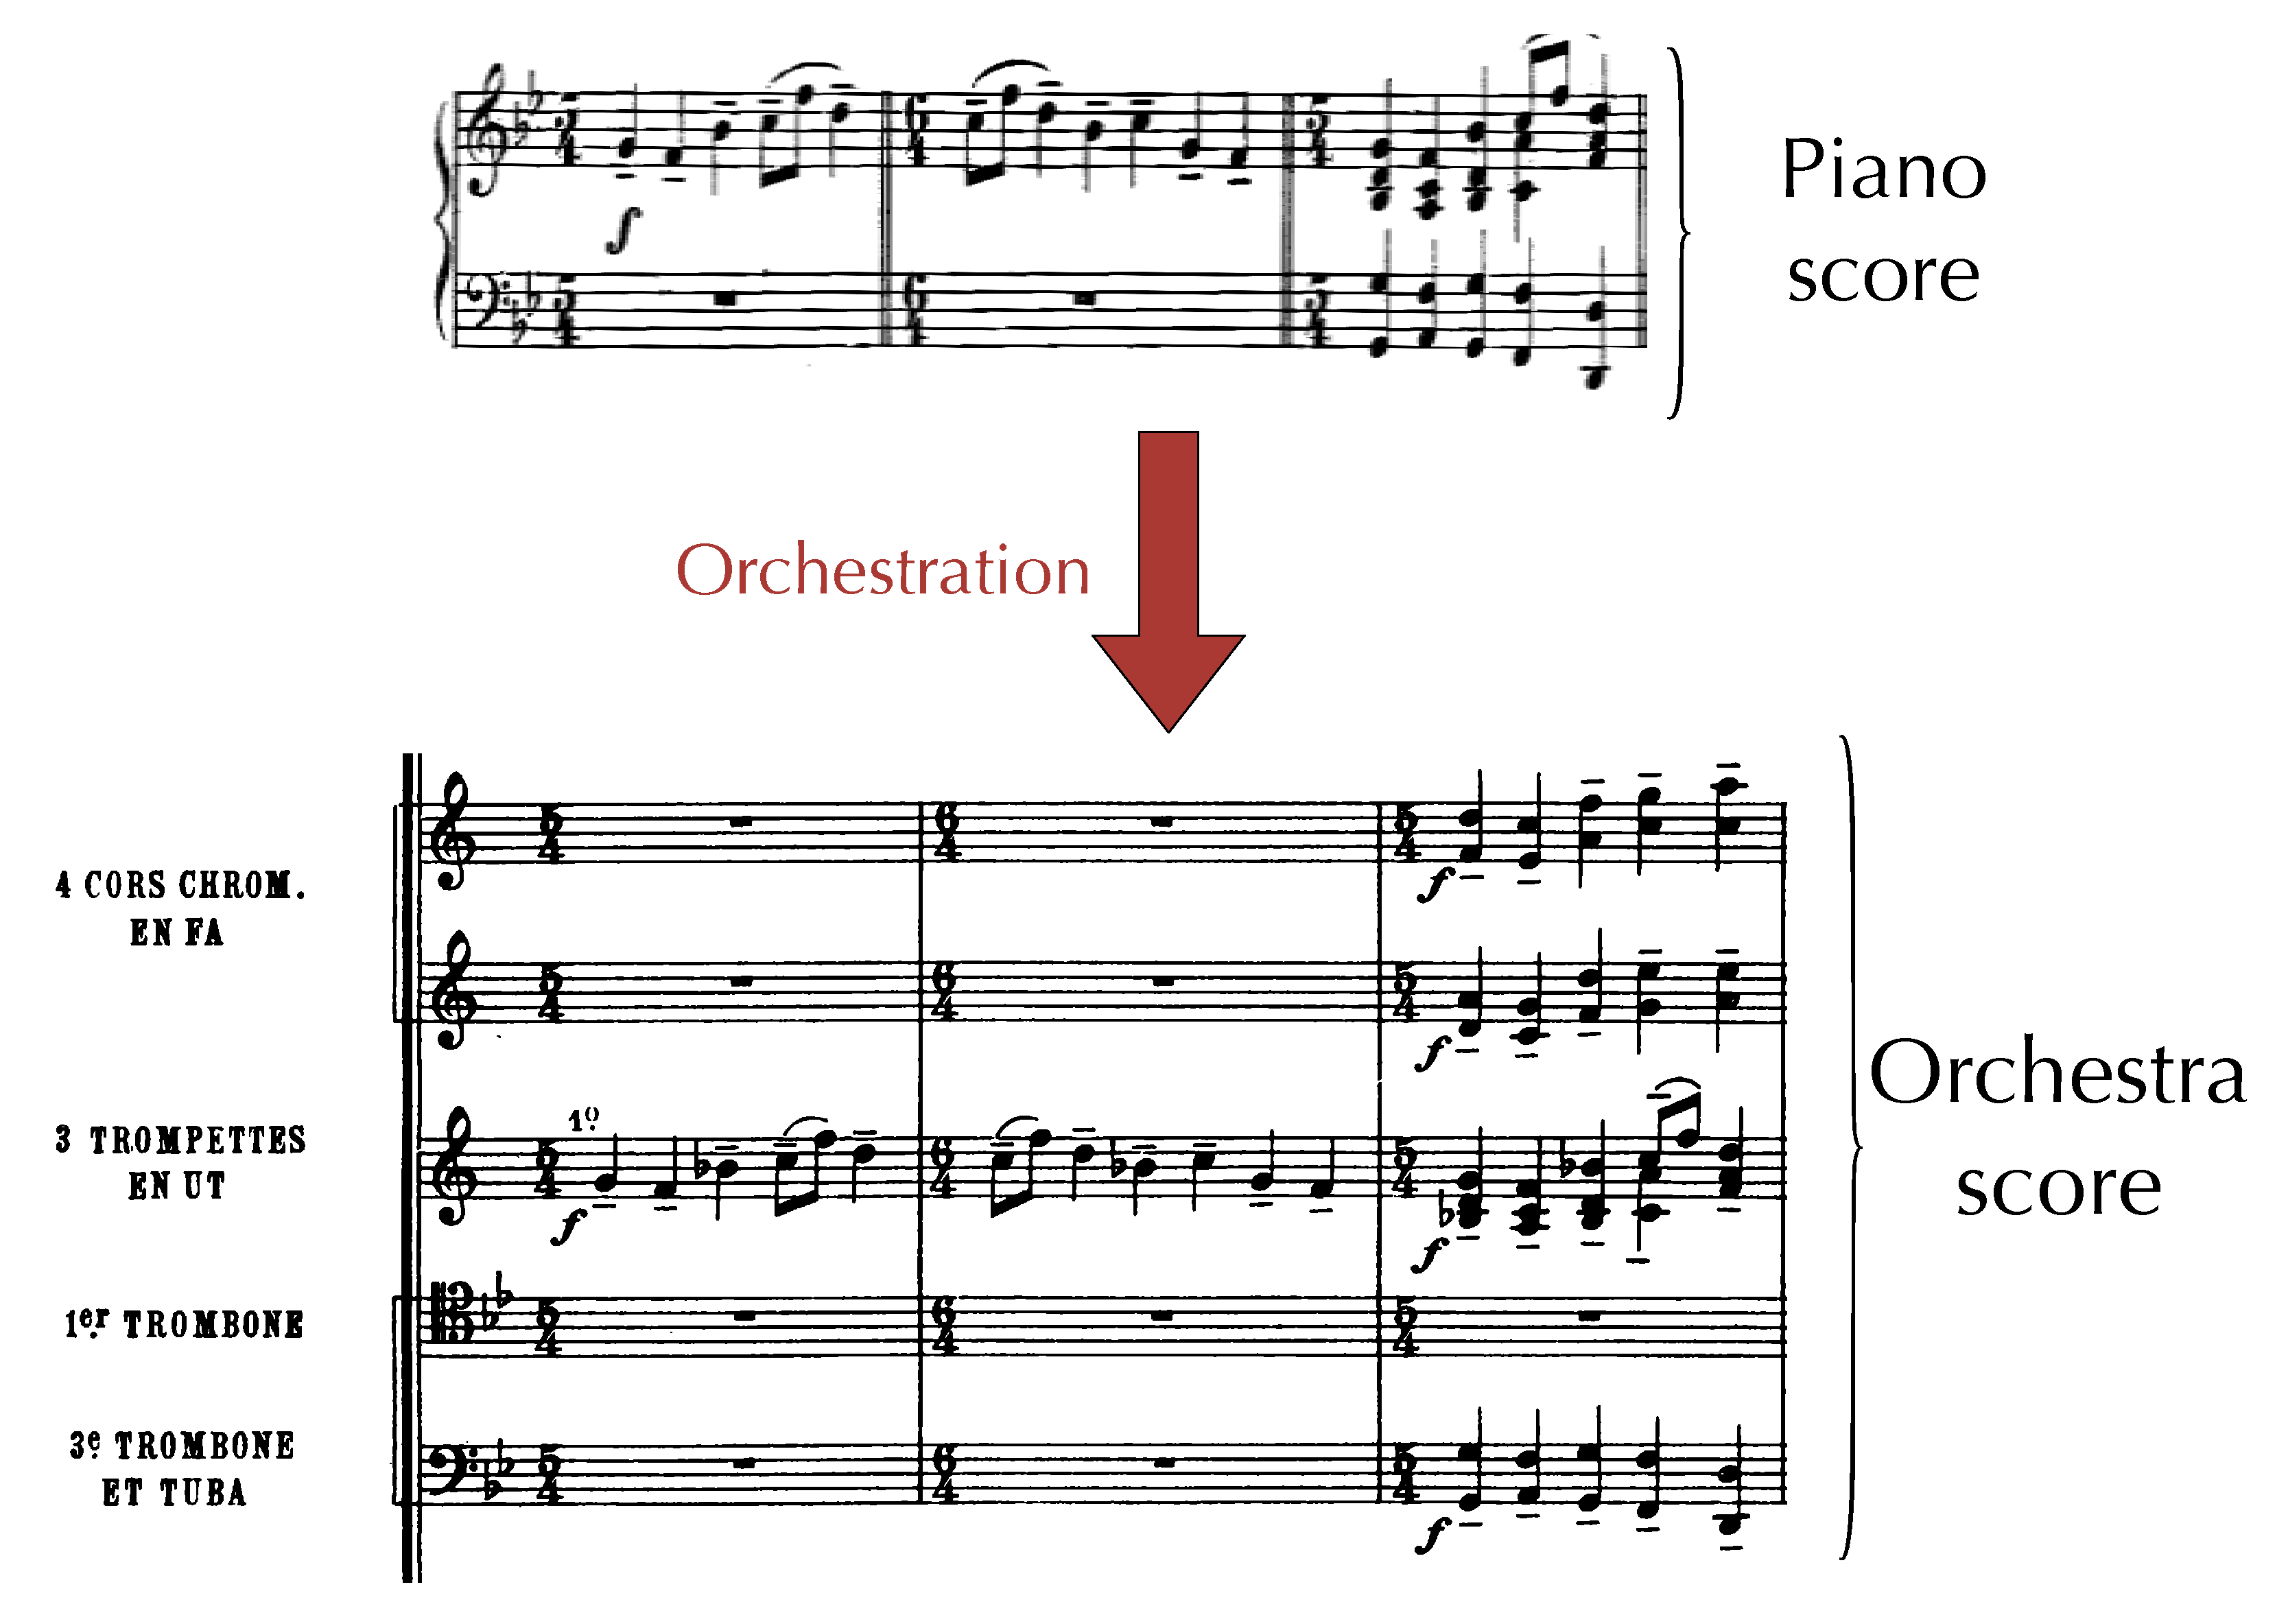
\includegraphics[scale=0.2]{orch}
\label{fig:orch}
\caption{\textit{Projective orchestration}. A piano score is extended (projected) on an orchestra. For one piano score, many acceptable orchestration exist. Our hypothesis is that a piano score is strongly correlated to any of the orchestration that could be produced from this piece.}
\end{figure}
\textit{Musical orchestration} is the subtle art of writing musical pieces for orchestra, by combining the spectral properties specific to each instrument in order to achieve a particular sonic goal. This complex discipline involves a wide set of intricate mechanisms, most of which have not yet been satisfactorily theorized. Indeed, famous composers often conjectured that orchestration would mainly remain an empirical discipline, which could only be learned through experience and never axiomatized in books. Even if several famous musicians have written orchestration treatises \cite{berlioz_orch,koechli_orch}, those mostly remain recommendations and sets of existing orchestration examples from which one can draw inspiration.
We focus more specifically in this work on \textit{projective} orchestration, which is the transformation from a piano score to an orchestral piece \prettyref{fig:orch}. Many composers have worked in a projective manner, and a large amount of examples can be found in the repertoire. For instance, one of the most famous is the orchestration of \textit{Les tableaux d'une exposition}, a Modest Moussorgsky's piano piece, by Maurice Ravel.

% Automatic orch, state of the art
The objective in this work is to be able to automatically perform in real-time the \textit{projective} orchestration of a piano performance.
More specifically, our system takes in input a piano score and outputs an orchestral score.
The vast combinatorial set of instrument possibilities added to the complex temporal structure of polyphonic music make this problem a particularly daunting task. Several attempts to build an automatic orchestration system can be found in the literature. 

Orchestration can be viewed as assigning the different notes of the piano score to a certain number of instrument according to constraints over the number of instruments, their tessitura or a certain voice leading. Interpreting orchestration as a Constraint Solving Problem (CSP) lead to a first solution \cite{Truchet2011Constraint-Prog}. However, as Steven McAdams pointed it out, timbre is "a structuring force in music" \cite{mcadams2013timbre} in the sense that it should be used to emphasize the already existing structure of the original piano piece. We believe that a system built only on symbolic constraint will undoubtedly fail at grasping the harmonic, rhythmic and melodic structure of the original piano piece and thus propose an interesting orchestration.
\textit{Orchids} (\cite{Esling2010}) is an other interesting work set in an other paradigm called \textit{injective} orchestration. It consists in trying to reconstruct a target timbre for a small temporal frame. Its major drawback is that \textit{Orchids} can only orchestrate short frames (less than 10 seconds).
% Why statistical inference ?
In order to build an automatic orchestration system being able to work on a macro-temporal timescale while structuring the musical discourse, statistical inference appeared us to be a promising solution. Their should indeed exist strong correlation between the information contained in the original piano score and the orchestral rendering we want to produce. Statistical inference would allow us to extract rules from the vast knowledge embodied in the many orchestration proposed by famous composers over the years.

% Which model and why ?
We decided to work with a class of models called conditional models \cite{taylor2009composable}, which derive from a particular type of Markov Random Field called the Restricted Boltzmann Machine (RBM) \cite{fischer2014training}. While being able to model complex distributions through latent units, those models implement a notion of context which allow us to model the influence of the past over the present and of the piano over the orchestra.
Those models are generative which is a requirement in our case. If correctly trained on a training dataset, a model then has the ability to generate data that are similar, yet unseen, to those contained in the training set. This is through this mechanism that orchestral projection can be performed.

% Evaluation framework
We then propose in this article a new evaluation framework for the orchestral projection task in order to evaluate the different model previously introduced.  This evaluation rely on a frame-level predictive task based on an accuracy measure.
% Results -> LOP
The results of the proposed model are then presented. We picked out the best model and included it in a real-time orchestration system called \textit{LOP}.

This paper is organized as follows. In sections 2 we introduce the state of the art in conditional models through three well known models: the RBM, the CRBM and the \textit{FGCRBM}. The orchestration projection task is presented in the section 3 along with an evaluation framework based on a frame-level accuracy measure. The previously introduced models are then evaluated in this framework and the results displayed. The section 4 introduces a real-time \textit{projective} orchestration system using the presented architectures.

\section{State of the art}
\label{sec:state_of_the_art}
The three model we have used in our work are the Restricted Boltzmann Machine (RBM), the Conditional RBM (CRBM) and the Factored Gated Conditional RBM (\textit{FGCRBM}). They derive from the Graphical Probabilistic Model (GPM) theory and more specifically from a class of models called Markov Random Fields (MRF) (\cite{fischer2014training}). They are presented by increasing level of complexity, each model adding a new \textit{degree of freedom} to the previous one.

\subsection{Restricted-Boltzmann Machine}
\begin{figure}
\centering
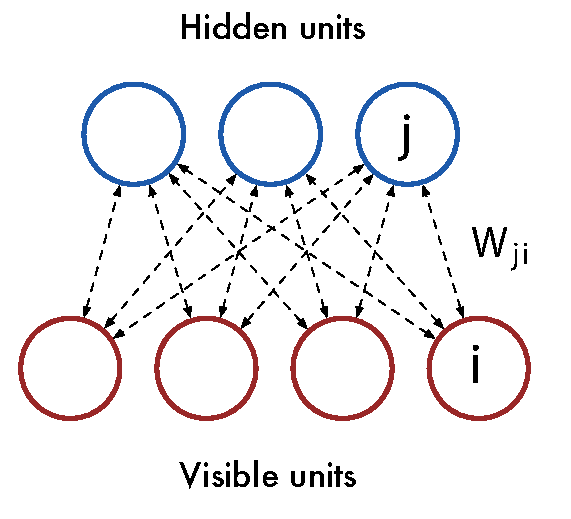
\includegraphics[scale=0.7]{RBM}
\caption{\textit{Restricted Boltzmann Machine}. The RBM is an energy-based model. Its energy function is computed from the values of weights that link nodes. Training an RBM consists in lowering the energy function around the example from a training set. Inference in this model is easy to perform since the hidden (resp. visible) units are independent from each others.}
\label{fig:RBM}
\end{figure}
A \gls{RBM} \cite{Hinton:2006:FLA:1161603.1161605} is an energy-based model that represent the joint distribution of a visible vector $\bm{v} = (v_{1},...,v_{m})$ and a hidden vector $\bm{h} = (h_{1},...,h_{n})$. This distribution is given by $p(\bm{v},\bm{h}) = \frac{\exp^{-E(\bm{v},\bm{h})}}{Z}$ where
\begin{equation}
E(\bm{v},\bm{h}) = - \sum_{i=1}^{m} a_{i} v_{i} - \sum_{j = 1}^{n} b_{j} h_{j} - \sum_{i=1}^{m} \sum_{j=1}^{n} v_{i} W_{ij} h_{j}
\end{equation}
and $Z = \sum_{v,h}\exp^{-E(v,h)}$ is a usually intractable partition function. $\bm{\Theta} = \left\lbrace \bm{W} , \bm{a} , \bm{b} \right\rbrace$ are the weights of the network.
Unfortunately, the gradient of the negative log-likelihood of a vector from the training database $\bm{v}^{(l)}$ is intractable because of the negative term in right-hand part of the equation \prettyref{eq:log-lik-grad} which involves a sum over all the possible combinations of the hidden units (alternatively all the possible configurations of the visible units). A training algorithm called \gls{CD} \cite{hinton2002training} rely on an approximation of the model driven term of this equation by running a k-step Gibbs chain to obtain a sample $\bm{v}^{(l,k)}$ \prettyref{eq:log-lik-grad}.
\begin{align}
\label{eq:log-lik-grad}
- \frac{\partial \ln(p(\bm{v^{(l)}}|\bm{\Theta}))}{\partial \bm{\Theta}}  &=  \mathbb{E}_{p(\bm{h}|\bm{v^{(l)}})} \left[ \frac{\partial E(\bm{v^{(l)}},\bm{h})}{\partial \bm{\Theta}} \right] - \mathbb{E}_{p(\bm{h},\bm{v})} \left[ \frac{\partial E(\bm{v},\bm{h})}{\partial \bm{\Theta}} \right]\\
& \approx \mathbb{E}_{p(\bm{h}|\bm{v^{(l)}})} \left[ \frac{\partial E(\bm{v^{(l)}},\bm{h})}{\partial \bm{\Theta}} \right] - \mathbb{E}_{p(\bm{h} | \bm{v^{(l,k)}})} \left[ \frac{\partial E(\bm{v^{(l,k)}},\bm{h})}{\partial \bm{\Theta}} \right]
\end{align}

Running a Gibbs sampling chain consists in alternatively sampling the hidden units knowing the visible units then the visible units knowing the inferred hidden units by using the marginal probabilities \prettyref{eq:marginal_RBM}.
\begin{align}
\label{eq:marginal_RBM}
p(v_{i}=1|\bm{h}) &= sigm \left( a_{i} + \sum_{j}W_{ij}h_{j} \right)\\
p(h_{j}=1|\bm{v}) &= sigm \left( b_{j} + \sum_{i}W_{ij}v_{i} \right)
\end{align}
where $sigm$ is the sigmoid function. Note that sampling from the marginal distribution is easy since visible units (respectively hidden units) are independent from each others. Hence, knowing the hidden units, all the visible units can be sampled in one step. This allows fast implementation through matrix operations and is known as \textit{block sampling}.
It has been proved \cite{bengio2009learning} that the samples we obtain after an infinite number of iteration will be drawn from the joint distribution of the visible and hidden units of our model. An other approximation consists in starting the Gibbs chain from the sample $\bm{v}^{(l)}$, which increases the convergence of the chain, and to limit the number of alternate sampling steps to a fixed number K. After evaluating the statistics (model driven terms), the parameters can be updated. The whole algorithm is called Contrastive Divergence-K (CD-K). In a RBM those update rules are given by
\begin{align}
\Delta W_{ij} &= <v_{i}h_{j} >_{data} - <v_{i}h_{j} >_{model}\\
\Delta a_{i} &= <v_{i}>_{data} - <v_{i}>_{model}\\
\Delta b_{j} &= <h_{j} >_{data} - <h_{j} >_{model}
\end{align}

\subsection{Conditional RBM}
\begin{figure}
\centering
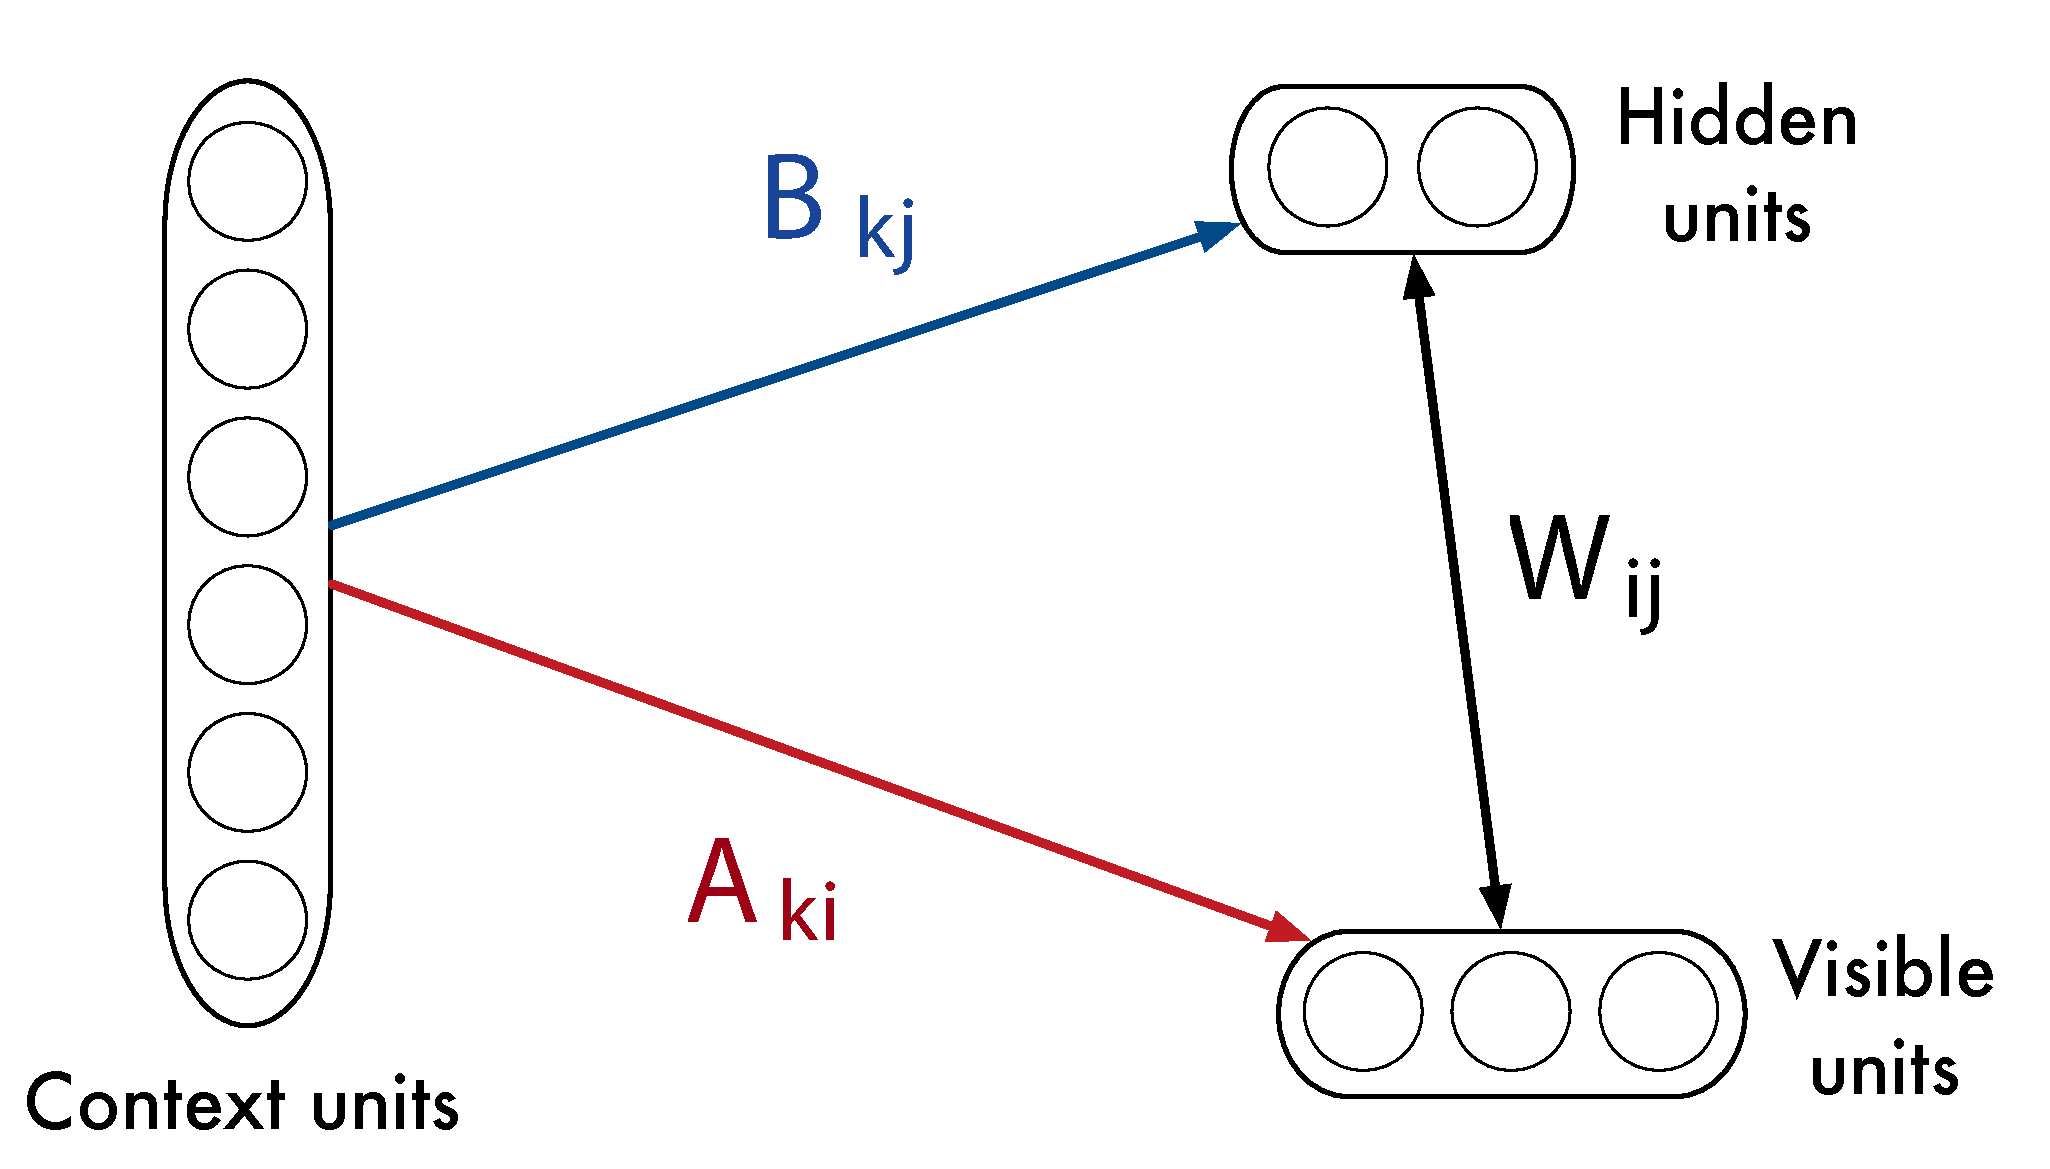
\includegraphics[scale=0.3]{CRBM_orchestration}
\caption{\textit{Conditional RBM}. A layer of context units is added to the standard RBM architectures. Those context units linearly modify the bias of both visible and hidden units.}
\end{figure}
The \gls{CRBM} model (\cite{taylor2009composable}) is an extension of the \gls{RBM}. A dynamic bias is added to the static bias of the visible ($\bm{a}$) and hidden $\bm{b}$ units. This dynamic bias linearly depends on a set of unit called context units $(\bm{x})$.
To model time series, if we consider that the visible units $\bm{v}(t)$ represent the current time frame, those context units can be defined as the concatenation of the N last time frames $\bm{x}(t) = \left( v_{1}^{(t)} , ... , v_{m}^{(t)}, ... , v_{1}^{(t-N)} ... , v_{m}^{(t-N)} \right)$, where N denotes the order of the model.
The energy function of the Conditional RBM is given by \prettyref{eq:energy_CRBM}
\begin{equation}
\label{eq:energy_CRBM}
E(\bm{v}(t),\bm{h}(t)|\bm{x}(t)) = - \sum_{i} \hat{a}_{i}(t)v_{i}(t) - \sum_{ij}W_{ij}v_{i}(t)h_{j}(t) - \sum_{j} \hat{b}_{j}(t)h_{j}(t)
\end{equation}
where the biases are defined by 
\begin{align*}
\hat{a}_{i}(t) &= a_{i} + \sum_{k}A_{ki}x_{k}(t)\\
\hat{b}_{j}(t) &= b_{j} + \sum_{k}B_{kj}x_{k}(t)
\end{align*}

This model can be trained by contrastive divergence, since the marginal probability of visible and hidden units are the same as in the RBM, while replacing the static biases by the dynamics biases.
The following updates rules are obtained
\begin{align}
\Delta W_{ij} 	&= <v_{i}h_{j} >_{data} - <v_{i}h_{j} >_{model}\\
\Delta a_{i}		&= <v_{i}>_{data} - <v_{i}>_{model}\\
\Delta b_{j}		&= <h_{j} >_{data} - <h_{j} >_{model}\\
\Delta A_{ik} 	&=<v_{i}x_{k} >_{data} - <v_{i}x_{k} >_{model}\\
\Delta B_{jk} 	&= <h_{j}x_{k} >_{data} - <h_{j}x_{k} >_{model}\\
\end{align}

\subsection{Factored Gated Conditional RBM}
\begin{figure}
\centering
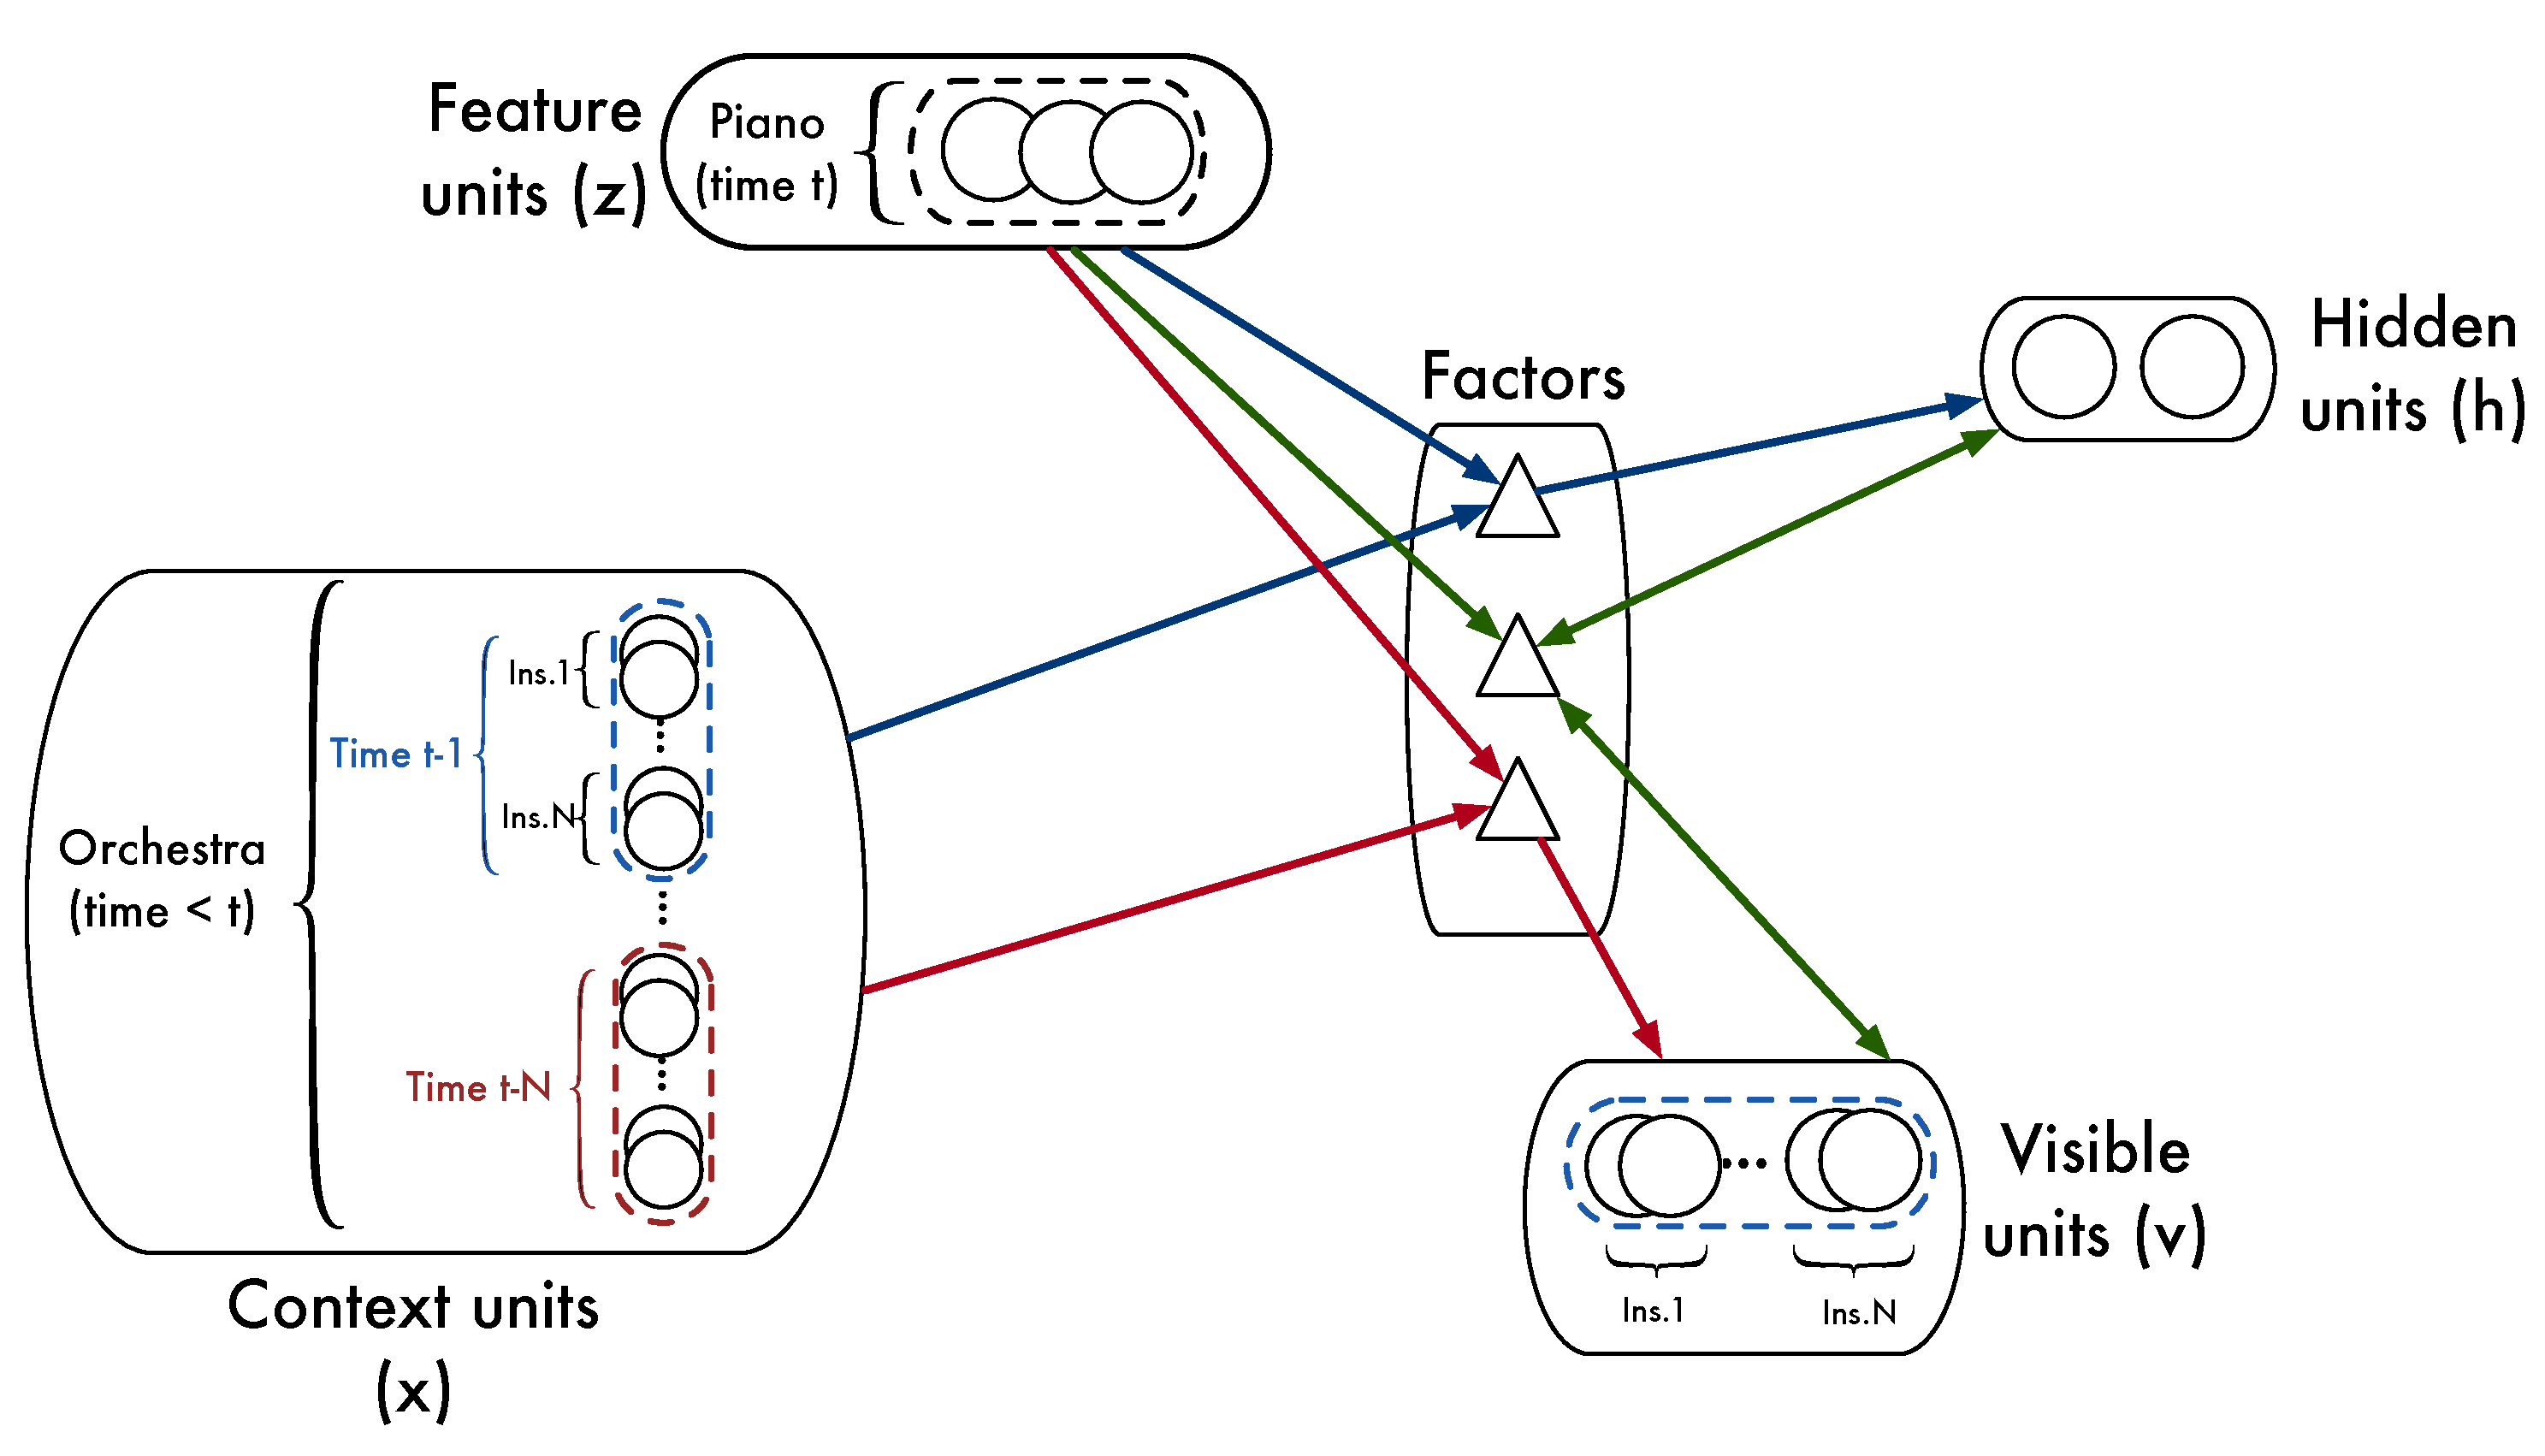
\includegraphics[scale=0.25]{FGCRBM_orchestration}
\caption{\textit{FGCRBM} model. The features units ($bm{z}$) modify the energy landscape of the model by a multiplicative influence over the weights $\bm{A}$, $\bm{B}$ and $\bm{W}$. Here, the role of each units in order to perform orchestration is indicated.}
\label{fig:FGCRBM}
\end{figure}
The Factored Gated Conditional RBM model \cite{taylor2009factored} proposes to extend the Conditional RBM model by adding a layer of feature units $\bm{z}$ which modulate the weights of the conditional architecture in a multiplicative way. Hence, the weights of the networks become $\bm{\Theta} = \left\lbrace \bm{W} , \bm{A} , \bm{B} , \bm{a} , \bm{b} \right\rbrace$, where $\bm{W} = (W)_{ijl}$, $\bm{A}=(A)_{ikl}$ and $\bm{B}=(B)_{jkl}$ are three dimensional tensors.

This multiplicative influence can be understood as a modification of the energy landscape of the model. Each configuration of the feature units defines a new energy function of the simple CRBM model defined by the other units ($\bm{v}$, $\bm{h}$, and $\bm{x}$). Since the number of parameters to train becomes high, the three dimensional tensors can be factorized into a product of three matrices by including factor units indexed by $f$ : $W_{ijl} = W_{if} . W_{jf} . W_{lf}$.
The energy function of this Factored Gated Conditional RBM is then given by
\begin{equation}
E(\bm{v}(t),\bm{h}(t)|\bm{x}(t),\bm{z}(t)) = -\sum_{f}\sum_{ijl} W_{if}^{v} W_{jf}^{h} W_{lf}^{z} v_{i}(t) h_{j}(t) z_{l}(t) 
- \sum_{i} \hat{a}_{i}(t)v_{i}(t) - \sum_{j} \hat{b}_{j}(t)h_{j}(t)
\end{equation}
where the dynamic biases of the visible and hidden units are defined by
\begin{equation}
\hat{a}_{i}(t) = a_{i} + \sum_{m} \sum_{kl}A_{im}^{v}A_{km}^{x}A_{lm}^{z}x_{k}(t)z_{l}(t)
\end{equation}
\begin{equation}
\hat{b}_{j}(t) = b_{j} + \sum_{n} \sum_{kl}B_{jn}^{h}B_{kn}^{x}B_{ln}^{z}x_{k}(t)z_{l}(t)
\end{equation}

The \textit{FGCRBM} model can be trained by contrastive divergence which lead to the following update rules for the parameter
\begin{align*}
\Delta b_{i}^{(v)} &= <v_{i}>_{data} - <v_{i}>_{model}\\
\Delta b_{j}^{(h)} &= <h_{j} >_{data} - <h_{j} >_{model}\\
\Delta W_{if}^{v} &= <v_{i}\sum_{j} W_{jf} h_{j} \sum_{l} W_{lf} z_{l}>_{data} - <v_{i}W_{jf} h_{j} \sum_{l} W_{lf} z_{l} >_{model}\\
\Delta W_{jf}^{h} &= <h_{j}\sum_{i}W_{if}v_{i} \sum_{l} W_{lf} z_{l}>_{data} - <h_{j}\sum_{i}W_{if}v_{i} \sum_{l} W_{lf} z_{l}>_{model}\\
\Delta W_{lf}^{z} &= <z_{l}\sum_{i}W_{if}v_{i} \sum_{j} W_{jf}h_{j}>_{data} - <z_{l}\sum_{i}W_{if}v_{i} \sum_{j} W_{jf}h_{j}>_{model}\\\Delta A_{im}^{v} &= <v_{i}\sum_{k}A_{km}x_{k} \sum_{l}A_{lm}z_{l}>_{data} - <v_{i}\sum_{k}A_{km}x_{k} \sum_{l}A_{lm}z_{l}>_{model}\\
\Delta A_{km}^{x} &= <x_{k}\sum_{i}A_{im}v_{i} \sum_{l}A_{lm}z_{l}>_{data} - <x_{k}\sum_{i}A_{im}v_{i} \sum_{l}A_{lm}z_{l}>_{model}\\
\Delta A_{lm}^{z} &= <z_{l} \sum_{i}A_{im}v_{i} \sum_{k}A_{km}x_{k}>_{data} - <z_{l} \sum_{i}A_{im}v_{i} \sum_{k}A_{km}x_{k}>_{model}\\
\Delta B_{jn}^{z} &=  <h_{j} \sum_{k}B_{kn}x_{k} \sum_{l}B_{ln}z_{l}>_{data} - <h_{j} \sum_{k}B_{kn}x_{k} \sum_{l}B_{ln}z_{l}>_{model}\\
\Delta B_{kn}^{z} &= <x_{k} \sum_{j}B_{jn}h_{j} \sum_{l}B_{ln}z_{l}>_{data} - <x_{k} \sum_{j}B_{jn}h_{j} \sum_{l}B_{ln}z_{l}>_{model}\\
\Delta B_{ln}^{z} &= <z_{l} \sum_{j}B_{jn}h_{j} \sum_{k}B_{kn}x_{k}>_{data} - <z_{l} \sum_{j}B_{jn}h_{j} \sum_{k}B_{kn}x_{k}>_{model}
\end{align*}

\subsection{Generative models}
\begin{figure}
\centering
\includegraphics[scale=0.3]{FGCRBM_sampling}
\caption{\textit{Sampling in a FGCRBM}. Context and Features units are respectively clamped to the last ($t-1$ to $t-N$) orchestral frames and the current ($t$) piano frame. Visible units are randomly initialized. Then, several Gibbs sampling step are performed, in our case 40.}
\label{fig:FGCRBM_sampling}
\end{figure}
%% Role des unités conditionelles et tout le tralala dans les modèles
The previously introduced models are generative. If a model has been correctly trained, its distribution approximates the underlying distribution of the training data. It is then possible to sample from this distribution in order to generate data that are similar to the data of the training set (\prettyref{fig:FGCRBM_sampling}).
The generation process can be described as follow. After randomly setting the visible units vector (for each index $i$, $\bm{v}_{i} \sim \mathcal{U}(0,1)$), alternate Gibbs sampling is performed in order to approximate the joint distribution of the hidden and visible units conditionally on the context units. Given the context units, one step of alternate Gibbs sampling consists in sampling the hidden units knowing the visible, then sampling the visible units knowing the hidden. In theory the visible sample obtained is from the model distribution after an infinite number of steps. If theoretically an infinite number of steps is necessary, in practice 20 to 100 steps are typically used. In our case, we obtained satisfying results with 40 sampling steps.

\subsection{Approximations}
In practice, several approximation are made both during training and generating phases. During the training phase, we have already seen the two approximations of the CD-K algorithm which consists in performing only a limited number of sampling steps, and starting the Gibbs chain with a sample from the training set.

\subsubsection{Mean-field values} An other common approximation can be made both during training and generating phases, when running the Gibbs chain in order to estimate the model-driven terms. In order to diminish the sampling noise mean-field values can be used for the visible units. This is not possible for the hidden units since it would violate the information bottleneck which is the fact that hidden units can only transmit a limited amount of information to the visible units \cite{hinton2010practical}. Indeed, hidden units can represent $2^{n}$ different states where $n$ is the number of hidden units. 

\subsubsection{Number of sampling steps} It is noteworthy that during the learning phase, only a small number of sampling step are performed (1 in our case, rarely more than 10) in the contrastive divergence algorithm. This is because the objective is simply to modify the energy of our model in order to increase the training set's likelihood under the model distribution. Indeed, it has been shown that even a small number of sampling steps guarantee to increase a lower bound over this quantity \cite{bengio2009learning}. When generating data, we really want to obtain a sample as close as possible to the distribution of the model and then a larger number of Gibbs sampling steps need to be performed.

\section{Projective orchestration}
Automatic orchestration suffers from the lack of quantitative evaluation framework. The different works on the domain mainly rely on qualitative evaluation (REF MAIS LESQUELLES ???).
To our best knowledge, there has not been any attempt in the automatic orchestration field to define a task associated to a performance measure. We propose here a first attempt in order to fill this gap by defining the orchestration projection task. This task consists in projecting a piano sequence on an orchestra. More precisely, it consists at each time $t$ to generate an orchestral vector knowing the piano frame $Piano(t)$ and the recent past of sequence of orchestral vectors $Orch(t-1),... Orch(t-N)$.
We define in this section an evaluation framework for projective orchestration based on a frame-level accuracy measure and then present the result of the previously introduced model in this framework.

\subsection{Formalization}
Conditional models allow to generate sequences of data under a certain context. Projective orchestration consists in producing an orchestral score conditionally on a piano score. In order to guarantee a certain continuity in the orchestration, voice leading for each instrument, the recent past of the orchestral sequence is also added in the contextual information.

\subsubsection{Data representation}
\label{sec:data_representation}
Before adapting the previously introduced models, the first step is to choose an adapted representation for the piano an orchestra scores.
\begin{figure}
\centering
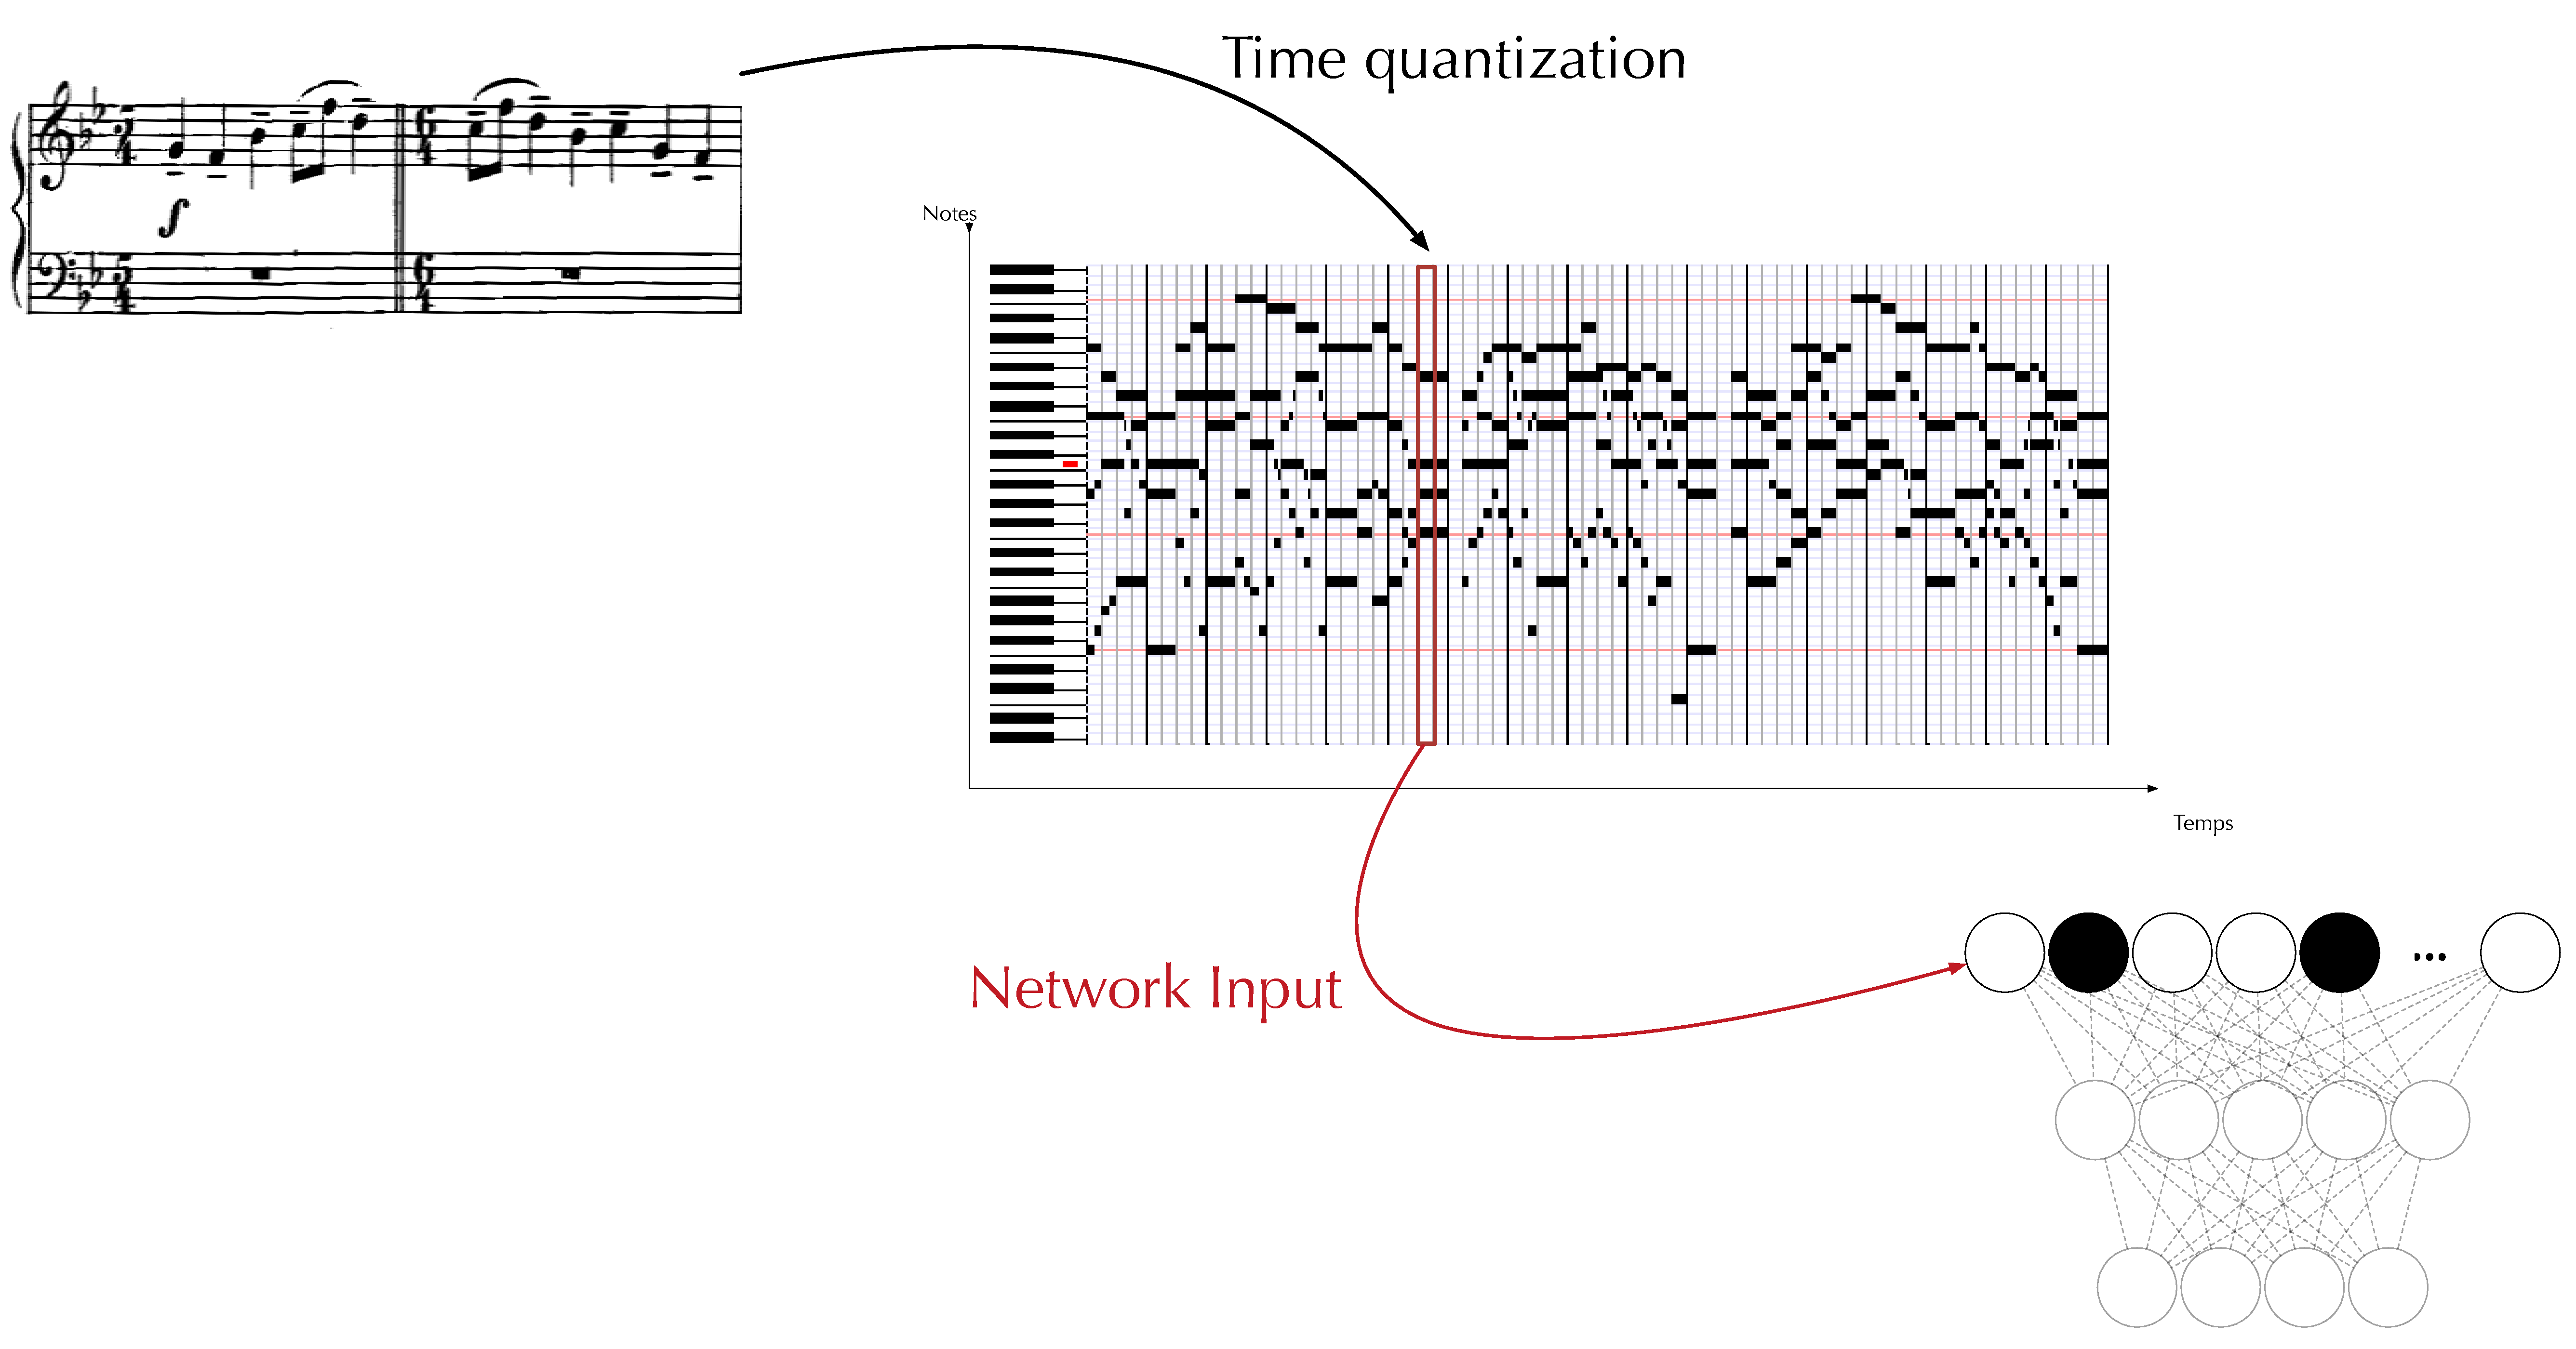
\includegraphics[scale=0.15]{representation_donnes}
\caption{\textit{Data representation for a single piano}. The pianoroll is a representation of musical events, discrete on both frequency scale (pitch) and the time scale (frames). A pitch $p$ at time $t$ can be either on or off, which is represented by a one or a zero on the pianoroll. To represent an orchestra, the pianorolls of each instruments are simply concatenated along the pitch dimension.}
\label{fig:pianoroll}
\end{figure}
To model sequences of symbolic music, the pianoroll representation is often used. 
This is a binary matrix $Pianoroll(p,t)$ which specify for a certain time quantisation if a pitch $p$ is played at time $t$.
The dynamics are ignored and each time frame is then represented by a binary vector $Pianoroll(t)$
This representation, usually defined for a single polyphonic instrument can easily be extended to an orchestra composed by N instruments by simply concatenating the pianoroll of each instrument over the pitch dimension.
\begin{equation}
Orch = 
\begin{bmatrix}
Instrument \ 1 \\
Instrument \ 2\\
\vdots\\
Instrument \ N\\
\end{bmatrix}
\end{equation}
Each instrument has a different playing range and the size of the pitch dimension is different for each instrument, limited to the pitch observed in the training dataset. For the piano score, the number of pitch is limited to $88$ which is then number of keys on a piano keyboard.
Note that we respect the usual simplifications used when writing orchestral scores which consists in grouping all the instruments of a same section. For instance, the section \textit{violin 1}, composed by many instrumentalists (10 or more), is represented as a unique instrument.
For a sequence of music of length $T$ and with $N$ instruments, $Orch$ is then a matrix of dimension $T \times \sum_{n=1}^{N} range(n)$. 

In our framework we chose 14 instruments indexed by :
\begin{tabular}{l l l l l}
1. Violin & & 6. Timpani & & 11. Oboe\\
2. Viola & & 7. Trumpet & & 12. Bassoon\\
3. Cello & & 8. Trombone & & 13. Clarinet\\
4. Double-bass & & 9. Tuba & & 14.Flute\\
5. Harp & & 10. French horn &\\
\end{tabular}

\subsubsection{Modeling orchestral sequences}
This data representation can be directly used in the previously introduced conditional models.
In the CRBM model, we consider that the visible units represent the orchestral vector for the time frame $t$, conditional units are be used to model the influence of the past orchestral vectors $Orch(t-1) , ... , Orch(t-N)$ and the influence of the piano frame at time $Piano(t)$ over the visible units. The context units are then defined by the concatenation of the past orchestral frames and the current piano frame
$ Context(t) = \left[ Piano(t)^{T} , Orch(t-1)^{T} , ... , Orch(t-N)^{T}\right]^{T}$.

The \textit{FGCRBM} model allows to separate the influence of the current piano frame and the past orchestral frames. The current piano frame defines the feature units ($z$) $ Features(t) = Piano(t)^{T} $, and the concatenation of the past orchestral frames define the context units ($x$) $ Context(t) = \left[ Orch(t-1)^{T} , ... , Orch(t-N)^{T} \right]^{T}$ (\prettyref{fig:FGCRBM}).

One might be surprised that for each time frame $t$, we do not restrain the possible pitches of each instrument to the pitches seen in the piano score at the same time $t$. This i because orchestrating a piano score can not be reduced to the simple projection of the notes that are already written on the piano score. Instead, the harmonic structure is often densified by adding extra notes, from a simple octaviation to an harmonic expansion (more complex chords with a more specific colour), the melody might be doubled by several instruments at different octave or the rhythmic structure slightly modified (held note instead of a staccato).

\subsection{Evaluation}
Building a quantitative evaluation framework for generative models is rarely straightforward, especially since computing the likelihood of a test sample is intractable in the models we used. In music automatic generation, a common practice consists in defining an auxiliary task. The most frequently task is a predictive task based on a frame-level accuracy that can be easily extended to the orchestral inference task \cite{DBLP:journals/corr/LiuR14a,boulanger2012modeling,lavrenko2003polyphonic}.
\subsubsection{Frame-level accuracy}
The frame level accuracy of a model over a testing set is defined as the mean value of the accuracy measured for each time frame. For each time frame, we try to predict the orchestral frame $\hat{Orch}(t)$ knowing the recent past $Orch(t-1),...,Orch(t-N)$ and the piano frame $Piano(t)$ and compare it to the original frame $Orch(t)$. The accuracy measure the difference between the predicted and original frames \cite{boulanger2012modeling,DBLP:journals/corr/LiuR14a}
\begin{equation}
\text{Accuracy}  = \frac{TP(t)}{TP(t) + FP(t) + FN(t)}
\label{eq:accuracy}
\end{equation}
where $TP(t)$ is the number of notes correctly predicted (true positives). $FP(t)$ is the number of notes predicted which are not in the original sequence (false positive) and $FN(t)$ is the number on unreported notes (false negative). 

Instead of binary values, activation probabilities are used for the predicted samples in order to reduce the sampling noise. In the case this probability is intractable, one should sample many predicted frames for each time frame and compute the mean value of those samples.

\subsubsection{Event-level accuracy}
A major flaw in the frame-level accuracy measure is its dependence to the rhythmic quantization chosen. Indeed, when the quantization become too small, it becomes highly probable that a frame is simply repeated at the next time frame. Hence, the best predictive model is simply a model which predict that the next time frame is the same as the frame $t-1$. This is not a desirable behaviour, and we propose an evaluation based on an event-level to address that issue.

A musical event is defined as a change in the orchestral score, either a note being switched on or off. The predictive event-level accuracy measure relies on the same accuracy measure previously defined \prettyref{eq:accuracy}. The only difference is that it occurs at each new event instead of each new time frame. Since the task is slightly different, the training phase has been consequently changed so that a model is trained only on new event frames.

% Be careful, event level not on the context

\subsection{Database}
We used a parallel database of piano scores and their orchestration by famous composers. The database consists of 76 \textit{XML} files. Given the complexity of the distribution we wanted to model and the reduced size of the database we have accessed to, we decided to keep as a test dataset only the last half of one track from our database. Hence 75 and a half files were used to train our model. We chose to do so in order to have the best generation ability.
The contrastive-divergence algorithm has been applied on mini-batches of size $100$ during the training phase. Thus we obtained $335$ mini-batches for the frame-level measure, and $89$ for the event-level measure.
For each instrument, the pitch range is reduced to the \textit{tessitura} observed in the training dataset (\label{sec:data_representation}). We used a rhythmic quantization of 8 frames per beat.

\subsection{Results}
We evaluated the \textit{CRBM} and \textit{FGCRBM} previously presented \prettyref{sec:state_of_the_art} in both the frame-level and event-level frameworks. Those two models are compared to a random prediction of each frame and to a simple model that outputs the previous frame as the current frame prediction (i.e. a untrained 1 order linear predictor). The results are presented in the following tables \pretryref{fig:result_frame} and \pretryref{fig:result_event}.

\begin{figure}
\centering
\begin{tabular}{c c}
\hline
\multirow{2}{*}{Model} & Orchestral Frame-level Acc \%\\
& DOSIM \\
\hline
Random & 0.51\%\\ 
Repeat & 93.25\%\\ 
\hline \hline
CRBM & 45.07\%\\ 
FGCRBM & 2.05\%\\ 
\end{tabular}
\caption{Frame-level expected accuracy for various musical models}
\label{fig:result_frame}
\end{figure}

\begin{figure}
\centering
\begin{tabular}{c c}
\hline
\multirow{2}{*}{Model} & Orchestral Event-level Acc \%\\
& DOSIM \\
\hline
Random & 0.50\%\\ 
Repeat & 93.25\%\\ 
\hline \hline
CRBM & 27.78\%\\ 
FGCRBM & \%\\ 
\end{tabular}
\caption{Frame-level expected accuracy for various musical models}
\label{fig:result_frame}
\end{figure}
%% C'est de la merde, même le edvent-level ça règle pas du tout le problème : soit on prédit l'event mais avec un context basé sur les frames, et dans ce cas là le modèle repeat est bon, soit on prends que les event mais ça n'a aucun sens (pas de rythme...)

\section{Live Orchestral Piano}


\section{Conclusion and future works}
% Better DB
% Change the data representation (Braids POWA)

\section{Typical references in new ACM Reference Format}
A paginated journal article \cite{Abril07}, an enumerated
journal article \cite{Cohen07}, a reference to an entire issue \cite{JCohen96},
a monograph (whole book) \cite{Kosiur01}, a monograph/whole book in a series (see 2a in spec. document)
\cite{Harel79}, a divisible-book such as an anthology or compilation \cite{Editor00}
followed by the same example, however we only output the series if the volume number is given
\cite{Editor00a} (so Editor00a's series should NOT be present since it has no vol. no.),
a chapter in a divisible book \cite{Spector90}, a chapter in a divisible book
in a series \cite{Douglass98}, a multi-volume work as book \cite{Knuth97},
an article in a proceedings (of a conference, symposium, workshop for example)
(paginated proceedings article) \cite{Andler79}, a proceedings article
with all possible elements \cite{Smith10}, an example of an enumerated
proceedings article \cite{VanGundy07},
an informally published work \cite{Harel78}, a doctoral dissertation \cite{Clarkson85},
a master's thesis: \cite{anisi03}, an online document / world wide web resource \cite{Thornburg01}, \cite{Ablamowicz07},
\cite{Poker06}, a video game (Case 1) \cite{Obama08} and (Case 2) \cite{Novak03}
and \cite{Lee05} and (Case 3) a patent \cite{JoeScientist001},
work accepted for publication \cite{rous08}, 'YYYYb'-test for prolific author
\cite{SaeediMEJ10} and \cite{SaeediJETC10}. Other cites might contain
'duplicate' DOI and URLs (some SIAM articles) \cite{Kirschmer:2010:AEI:1958016.1958018}.
Boris / Barbara Beeton: multi-volume works as books
\cite{MR781536} and \cite{MR781537}.

% Appendix
\appendix
\section*{APPENDIX}
\setcounter{section}{1}
In this appendix, we measure
the channel switching time of Micaz [CROSSBOW] sensor devices.
In our experiments, one mote alternatingly switches between Channels
11 and 12. Every time after the node switches to a channel, it sends
out a packet immediately and then changes to a new channel as soon
as the transmission is finished. We measure the
number of packets the test mote can send in 10 seconds, denoted as
$N_{1}$. In contrast, we also measure the same value of the test
mote without switching channels, denoted as $N_{2}$. We calculate
the channel-switching time $s$ as
\begin{eqnarray}%
s=\frac{10}{N_{1}}-\frac{10}{N_{2}}. \nonumber
\end{eqnarray}%
By repeating the experiments 100 times, we get the average
channel-switching time of Micaz motes: 24.3$\mu$s.

\appendixhead{ZHOU}

% Acknowledgments
\begin{acks}
The authors would like to thank Dr. Maura Turolla of Telecom
Italia for providing specifications about the application scenario.
\end{acks}

% Bibliography
\bibliographystyle{ACM-Reference-Format-Journals}
\bibliography{../../biblio}
                             % Sample .bib file with references that match those in
                             % the 'Specifications Document (V1.5)' as well containing
                             % 'legacy' bibs and bibs with 'alternate codings'.
                             % Gerry Murray - March 2012

% History dates
\received{February 2007}{March 2009}{June 2009}

% Electronic Appendix
\elecappendix

\medskip

\section{This is an example of Appendix section head}

Channel-switching time is measured as the time length it takes for
motes to successfully switch from one channel to another. This
parameter impacts the maximum network throughput, because motes
cannot receive or send any packet during this period of time, and it
also affects the efficiency of toggle snooping in MMSN, where motes
need to sense through channels rapidly.

By repeating experiments 100 times, we get the average
channel-switching time of Micaz motes: 24.3 $\mu$s. We then conduct
the same experiments with different Micaz motes, as well as
experiments with the transmitter switching from Channel 11 to other
channels. In both scenarios, the channel-switching time does not have
obvious changes. (In our experiments, all values are in the range of
23.6 $\mu$s to 24.9 $\mu$s.)

\section{Appendix section head}

The primary consumer of energy in WSNs is idle listening. The key to
reduce idle listening is executing low duty-cycle on nodes. Two
primary approaches are considered in controlling duty-cycles in the
MAC layer.

\end{document}
% End of v2-acmsmall-sample.tex (March 2012) - Gerry Murray, ACM


